\section{Proposed Methodology}
\label{sec:methodology}

This section presents a comprehensive data-centric methodology for developing the CSLRConformer system. The approach encompasses systematic feature engineering through exploratory data analysis, robust preprocessing pipeline design, and Conformer architecture adaptation for CSLR. Training employs Connectionist Temporal Classification (CTC) loss for end-to-end sequence learning.

%-------------------------------------------------------------------------
\subsection{Exploratory Data Analysis and Keypoint Selection}

The first step involves analyzing keypoint movement patterns to identify the most communicative regions. For each keypoint, movement is quantified by calculating the total displacement across consecutive frames using Equation~\ref{eq:displacement}:

\begin{equation}
D_i = \sum_{t=1}^{T-1} \|\text{position}_i(t+1) - \text{position}_i(t)\|_2
\label{eq:displacement}
\end{equation}

The displacement calculation in Equation~\ref{eq:displacement} serves as a proxy for communicative activity, where higher values indicate more active keypoints. This approach is inspired by motion analysis techniques commonly used in gesture recognition \cite{huang2024video} and human activity analysis \cite{camgoz2018neural}.

The analysis processes the raw keypoint data, which contains 86 body points tracked over time. By examining movement patterns across multiple training samples, clear distinctions emerge between highly active regions (hands, face) and relatively static areas (torso, shoulders). As shown in Figure~\ref{fig:keypoint_movement_analysis}, the top 20 most active keypoints consistently correspond to hand and facial regions, validating the linguistic assumption that these areas carry the primary communicative load.

To ensure consistent data quality, DBSCAN clustering \cite{deng2020dbscan} identifies reliable keypoints by filtering outliers and tracking inconsistencies. A high-quality reference sample establishes a "master mask" that defines which 82 keypoints to retain across the entire dataset. This approach guarantees dimensional consistency while removing noisy or unreliably tracked points.

\begin{figure}
    \centering
    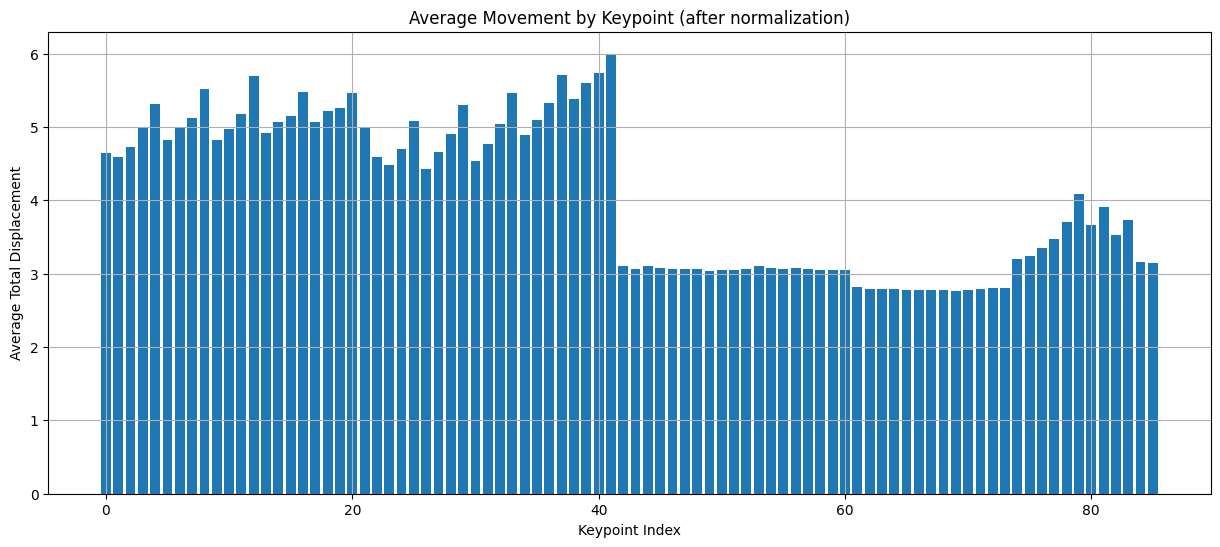
\includegraphics[width=1\linewidth]{keypoint_analysis.png}
    \caption{Movement analysis reveals that hand and facial keypoints exhibit significantly higher activity than body keypoints, confirming their communicative importance for sign language recognition.}
    \label{fig:keypoint_movement_analysis}
\end{figure}

%-------------------------------------------------------------------------
\subsection{Preprocessing Pipeline}

\subsubsection{Keypoint Filtering and Normalization}

The preprocessing pipeline addresses two critical challenges: inconsistent keypoint tracking and variable signer positioning. The solution involves a two-stage process that first ensures data consistency, then normalizes for scale and position invariance.

\textbf{Stage 1: Consistency Filtering}
Rather than processing each sample independently, the pipeline applies a single, consistent filter across the entire dataset. Using DBSCAN clustering \cite{deng2020dbscan} on a reference sample, reliable keypoints are identified and form a static mask. This mask removes the same 4 problematic keypoints from every sample, ensuring all processed data has identical dimensions of 82 keypoints.

\textbf{Stage 2: Frame-Level Normalization}
Each video frame undergoes normalization to handle different camera distances, angles, and signer positions. The process calculates a bounding box around all valid keypoints, then applies scale and translation normalization according to Equation~\ref{eq:normalization}:

\begin{equation}
\text{normalized\_keypoints} = \frac{\text{keypoints} - \text{bbox\_min}}{\text{scale}} - \text{center}
\label{eq:normalization}
\end{equation}

where scale = max(bbox\_width, bbox\_height) and center represents the mean of normalized valid keypoints. The normalization approach in Equation~\ref{eq:normalization} follows established pose normalization techniques \cite{thoker2021skeleton} and creates a standardized representation where the model learns relative keypoint relationships rather than absolute positions.

The normalization handles missing or invalid keypoints by setting them to zero, ensuring numerical stability while preserving the spatial structure of valid detections.

\begin{figure}
    \centering
    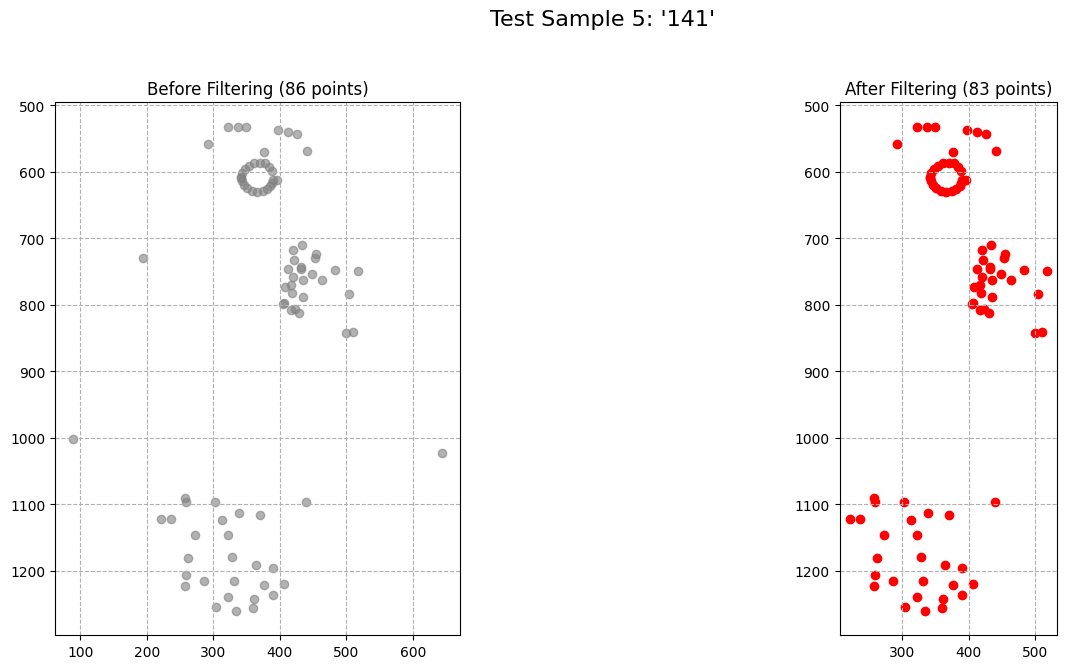
\includegraphics[width=1\linewidth]{460159971-10233a12-a7e4-450b-b069-51fd92ace2fd.png}
    \caption{Keypoint filtering process: Raw data (left) contains 86 keypoints with outliers, while filtered data (right) retains 82 reliable keypoints after DBSCAN-based consistency filtering.}
    \label{fig:outlier_filtering}
\end{figure}

The effectiveness of the two-stage filtering process is demonstrated in Figure~\ref{fig:outlier_filtering}, which shows the clear improvement in data quality after applying consistent filtering.

\subsubsection{Dynamic Feature Engineering}

Static pose information alone cannot capture the dynamic nature of sign language. The pipeline augments positional data with movement information by computing velocity and acceleration features using finite difference approximations \cite{torres2014automatic}.

\textbf{Position Features:} The 82 keypoints with x,y coordinates create a 164-dimensional base feature vector representing the current pose configuration.

\textbf{Velocity Features:} First-order temporal derivatives capture how keypoints move between frames. Using a 5-frame sliding window with convolution-based approximation, the system estimates movement speed for each keypoint using Equation~\ref{eq:velocity}:

\begin{equation}
\text{velocity}(t) = \frac{\text{position}(t+1) - \text{position}(t-1)}{2}
\label{eq:velocity}
\end{equation}

\textbf{Acceleration Features:} Second-order derivatives reveal how movement changes over time, capturing important dynamics like gesture initiation and deceleration patterns using Equation~\ref{eq:acceleration}:

\begin{equation}
\text{acceleration}(t) = \text{velocity}(t+1) - \text{velocity}(t-1)
\label{eq:acceleration}
\end{equation}

The velocity computation in Equation~\ref{eq:velocity} and acceleration calculation in Equation~\ref{eq:acceleration} employ central difference approximations that provide robust estimates of temporal derivatives while maintaining computational efficiency. This approach is consistent with motion analysis techniques used in gesture recognition \cite{huang2024video}.

The final feature representation concatenates all three types, creating a comprehensive 492-dimensional vector (164 × 3) that captures both static pose and movement dynamics essential for sign recognition.

%-------------------------------------------------------------------------
\subsection{CSLRConformer Architecture}

\subsubsection{Overall Design Philosophy}

The CSLRConformer adapts the standard Conformer architecture \cite{gulati2020conformer} specifically for sign language recognition challenges. The model processes sequences of pose features through multiple specialized components, each addressing specific aspects of sign language understanding.

\subsubsection{Architecture Components}

\textbf{Temporal Subsampling Module}
Sign language videos typically contain high frame rates that create computational challenges. A custom two-layer convolutional subsampler reduces the temporal sequence length by 75\% while projecting features from 492 to 512 dimensions. This design preserves essential temporal information while making attention computation tractable, following subsampling strategies established in speech recognition \cite{gulati2020conformer}.

\textbf{Positional Encoding}
Since attention mechanisms are inherently position-agnostic, sinusoidal positional encoding \cite{thoker2021skeleton} injects temporal order information. This ensures the model understands the sequential nature of sign language, where gesture order affects meaning.

\textbf{Data Augmentation for Robustness}
During training, SpecAugment \cite{park2019specaugment} randomly masks portions of the input to improve generalization. Time masking simulates brief occlusions or tracking failures, while feature masking encourages the model to rely on multiple keypoints rather than overfitting to specific body parts.

\textbf{Conformer Block Stack}
The core processing occurs through 8 Conformer blocks, each implementing a "sandwich" structure that balances local and global modeling \cite{gulati2020conformer}. Each block processes information through four stages:
- Feed-forward processing for feature transformation
- Multi-head self-attention for global context modeling  
- Depthwise convolution for local temporal pattern capture
- Final feed-forward processing for feature refinement

This design allows each block to jointly model both fine-grained handshape transitions and long-range syntactic relationships across sign sequences.

\textbf{Classification and Training}
The final linear layer projects hidden representations to the 1000-word vocabulary space. CTC loss \cite{graves2006connectionist} enables training without frame-level annotations by automatically learning alignment between input sequences and target glosses.

\begin{figure}
    \centering
    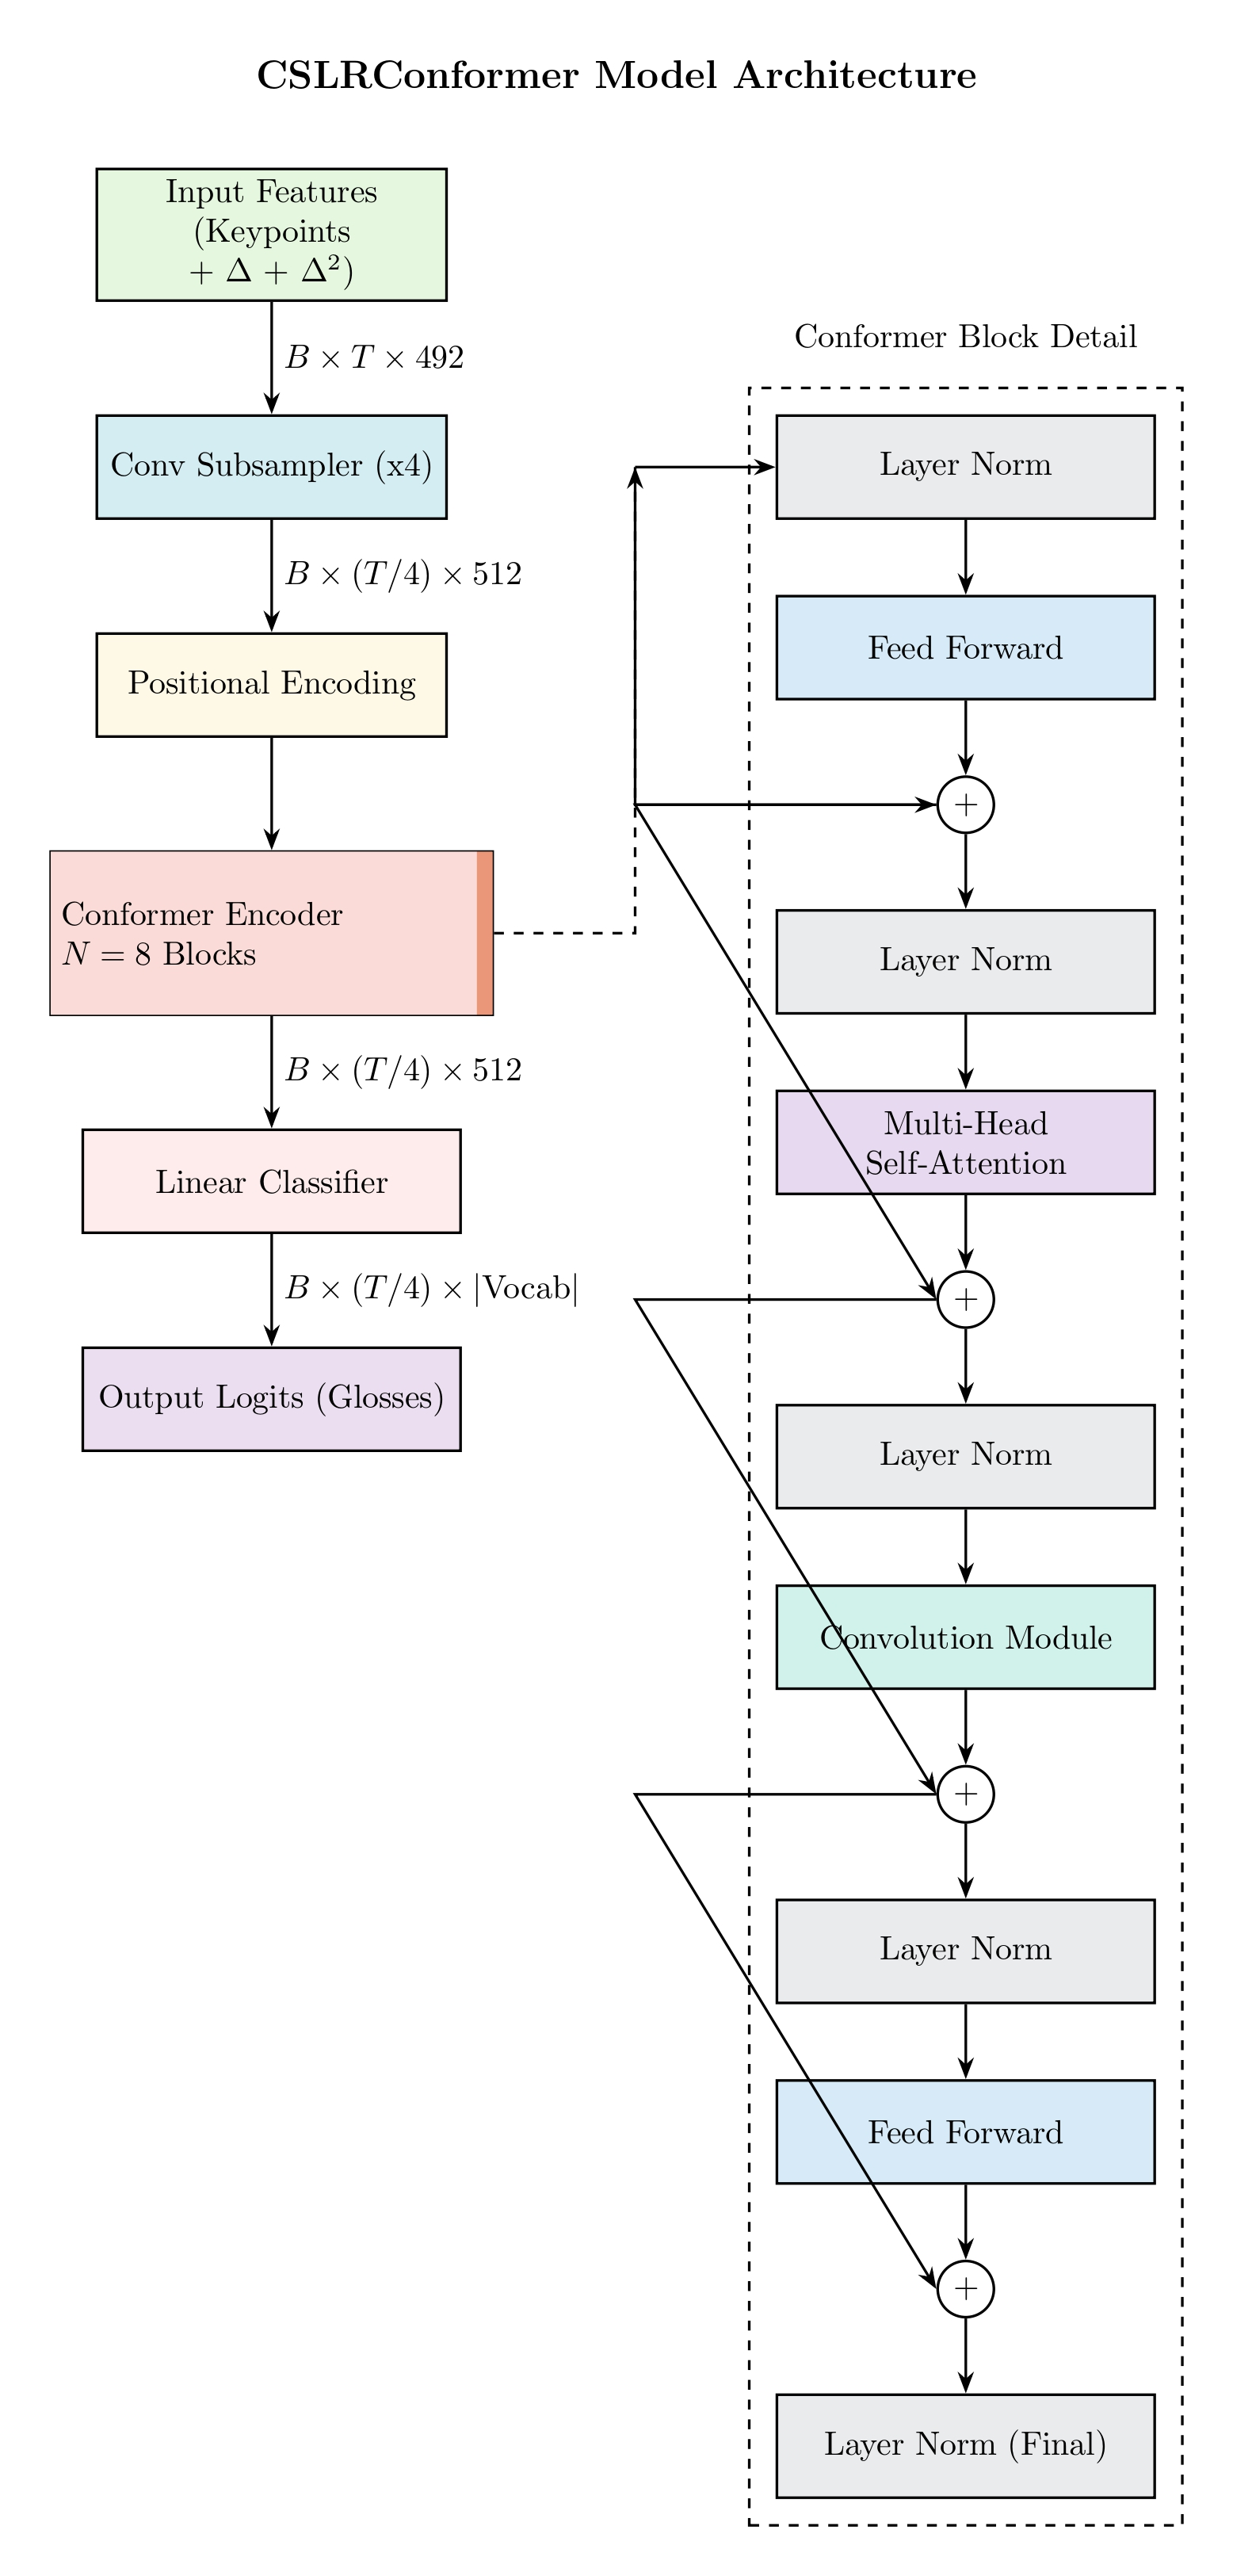
\includegraphics[width=0.75\linewidth]{model.jpg}
    \caption{CSLRConformer architecture processes keypoint sequences through subsampling, positional encoding, and 8 Conformer blocks before final classification. The hybrid design enables both local and global temporal modeling}
    \label{fig:cslr_conformer_architecture}
\end{figure}

The complete CSLRConformer architecture is illustrated in Figure~\ref{fig:cslr_conformer_architecture}, showing the flow from input keypoint sequences through the various processing stages to final gloss prediction.

\subsubsection{Training Strategy}
The training approach emphasizes stability through progressive learning (15-epoch warm-up followed by cosine annealing) and regularization (layer dropout, mixed precision training). Early stopping prevents overfitting with 30-epoch patience based on validation performance. This training strategy follows established practices in transformer-based sequence modeling \cite{gulati2020conformer}.